\documentclass[11pt,letterpaper]{article}

\usepackage{graphicx}
\usepackage{geometry}
\usepackage{amsmath}
\usepackage{hyperref}
\usepackage{url}
\usepackage{natbib}
\usepackage{booktabs}
\usepackage{xcolor}
\usepackage{listings}

\geometry{margin=1in}

\hypersetup{
  colorlinks=true,
  linkcolor=black,
  citecolor=black,
  urlcolor=black
}

\title{Longer Reasoning Chains Reduce Self-Check Agreement in Language Models}

\author{}

\date{}

\begin{document}

\maketitle

\begin{abstract}
Chain-of-thought (CoT) prompting has become the standard for eliciting reasoning from large language models, with a widely held assumption that longer reasoning traces produce more reliable answers. We challenge this assumption by introducing self-check divergence: the phenomenon where a model independent re-evaluation of a problem increasingly disagrees with its original CoT-derived answer as reasoning length increases. Through experiments on 1,156 GSM8K problems using MiniStral-3B, we measure three metrics across short, medium, and long CoT lengths: CoT accuracy, self-check accuracy, and self-check agreement rate. Our results reveal that long CoT traces produce the lowest agreement rate (54.8\%) compared to medium (75.6\%) and short (68.1\%), with a medium effect size (Cohen h = 0.27, p < 0.001). Surprisingly, agreement follows an inverted-U pattern mirroring accuracy, rather than the monotonic decline predicted by noise accumulation theory. We identify a consistency-accuracy gap at short lengths where models are accurate but internally inconsistent, and show that long CoT is harmful for both accuracy and reproducibility. These findings have direct implications for self-verification pipelines, suggesting that verification reliability decreases with reasoning length and that optimal CoT length for reliability differs from optimal length for accuracy.
\end{abstract}

\section{Introduction}

Chain-of-thought (CoT) prompting has transformed how we elicit reasoning from large language models (LMs). By asking models to generate intermediate reasoning steps before producing a final answer, CoT has achieved dramatic improvements on benchmarks ranging from arithmetic word problems to logical reasoning tasks \citep{Wei2022}. The success of CoT has spawned a family of verification-based methods---Chain-of-Verification \citep{Dhuliawala2023}, Self-Refine \citep{Madaan2023}, and self-consistency \citep{Wang2022}---that rely on the model ability to independently re-evaluate its own reasoning. These methods share a critical assumption: that a model can reliably check its own work, and that longer reasoning chains produce answers that are more verifiable.

We challenge this assumption by identifying a phenomenon we call \textbf{self-check divergence}: as CoT length increases beyond an optimal point, the agreement rate between a model CoT-derived answer and its independent self-check answer decreases sharply---even when the CoT answer is correct. This creates a self-verification paradox: the model own checking mechanism becomes less trustworthy precisely when it is most needed, on hard problems that require long reasoning chains.

The problem is concrete and measurable. When a model generates a long CoT trace to solve a math problem, each reasoning step introduces small amounts of noise: arithmetic slips, logical shortcuts, or factual approximations. When the same model is asked to independently re-evaluate the same problem without access to the original trace, it follows a different generative path. The accumulated noise from the longer original trace makes the model independent re-evaluation increasingly likely to disagree with the original answer, even when both the original and the re-evaluation are individually plausible.

This phenomenon matters for three reasons. First, it reveals a fundamental limitation in self-verification pipelines that are widely deployed to improve LLM reliability. If longer reasoning chains produce answers that the model itself cannot consistently reproduce when re-evaluating independently, then self-verification becomes less trustworthy on exactly the problems where it is most needed. Second, it suggests that the relationship between CoT length and reliability is not monotonic in the way commonly assumed---there may be an optimal CoT length that maximizes both accuracy and internal consistency. Third, it provides a new metric for evaluating model reasoning quality: self-check agreement rate, which captures a dimension of reliability that accuracy alone cannot measure.

Our work differs from prior research in a critical way. Zhou et al. \citep{Zhou2026} demonstrate that accuracy follows a pattern of diminishing returns with extended reasoning, showing that flip events where models abandon correct answers increase with token budget. However, they measure within-trace stability (a single trace growing longer), not cross-attempt reproducibility (two independent traces). Wu et al. \citep{Wu2025} show that accuracy follows an inverted-U curve with CoT length, but measure accuracy against ground truth, not internal consistency between reasoning and self-check. Wang et al. \citep{Wang2022} show that self-consistency improves accuracy through majority voting across samples, but measure agreement at fixed length only. No prior work measures self-check agreement rate as a function of CoT length, distinguishing between accuracy decline and internal consistency decline.

Our contributions are:

\begin{enumerate}
  \item \textbf{Self-check divergence metric.} We introduce a novel metric that measures the agreement rate between a model CoT-derived answer and its independent self-check answer as a function of CoT length, capturing a dimension of reasoning reliability that accuracy alone cannot measure.

  \item \textbf{Empirical validation.} We report the first experimental measurement of self-check divergence on 1,156 GSM8K problems \citep{Cobbe2021} across three CoT lengths and three difficulty tiers, finding that long CoT traces produce a 20.8 percentage-point drop in agreement rate relative to medium CoT (54.8\% vs.\ 75.6\%, Cohen h = 0.27, p < 0.001) \footnote{Code: \url{https://github.com/ai-inventor-papers/ai-invention-febf9b-longer-reasoning-chains-reduce-self/tree/main/round-2/evaluation-1}}.

  \item \textbf{Inverted-U pattern for agreement.} Contrary to our initial hypothesis of monotonic decline, we find that self-check agreement follows an inverted-U pattern mirroring accuracy: medium CoT maximizes both accuracy (82.3\%) and agreement (75.6\%), while short CoT exhibits a consistency-accuracy gap (83.2\% accuracy but only 68.1\% agreement), and long CoT collapses on both dimensions (49.9\% accuracy, 54.8\% agreement).

  \item \textbf{Difficulty-stratified analysis.} We show that the self-check divergence effect is strongest for hard problems (76.0\% to 50.7\% agreement drop from medium to long CoT) and persists across all difficulty tiers, suggesting that long CoT is universally harmful for reproducibility.

  \item \textbf{Theoretical framework.} We propose a noise accumulation model grounded in numerical analysis (error diffusion) and information theory (signal-to-noise degradation) to explain the observed patterns, with a revised account that accounts for the inverted-U pattern.
\end{enumerate}

\begin{figure}[!htbp]
  \centering
  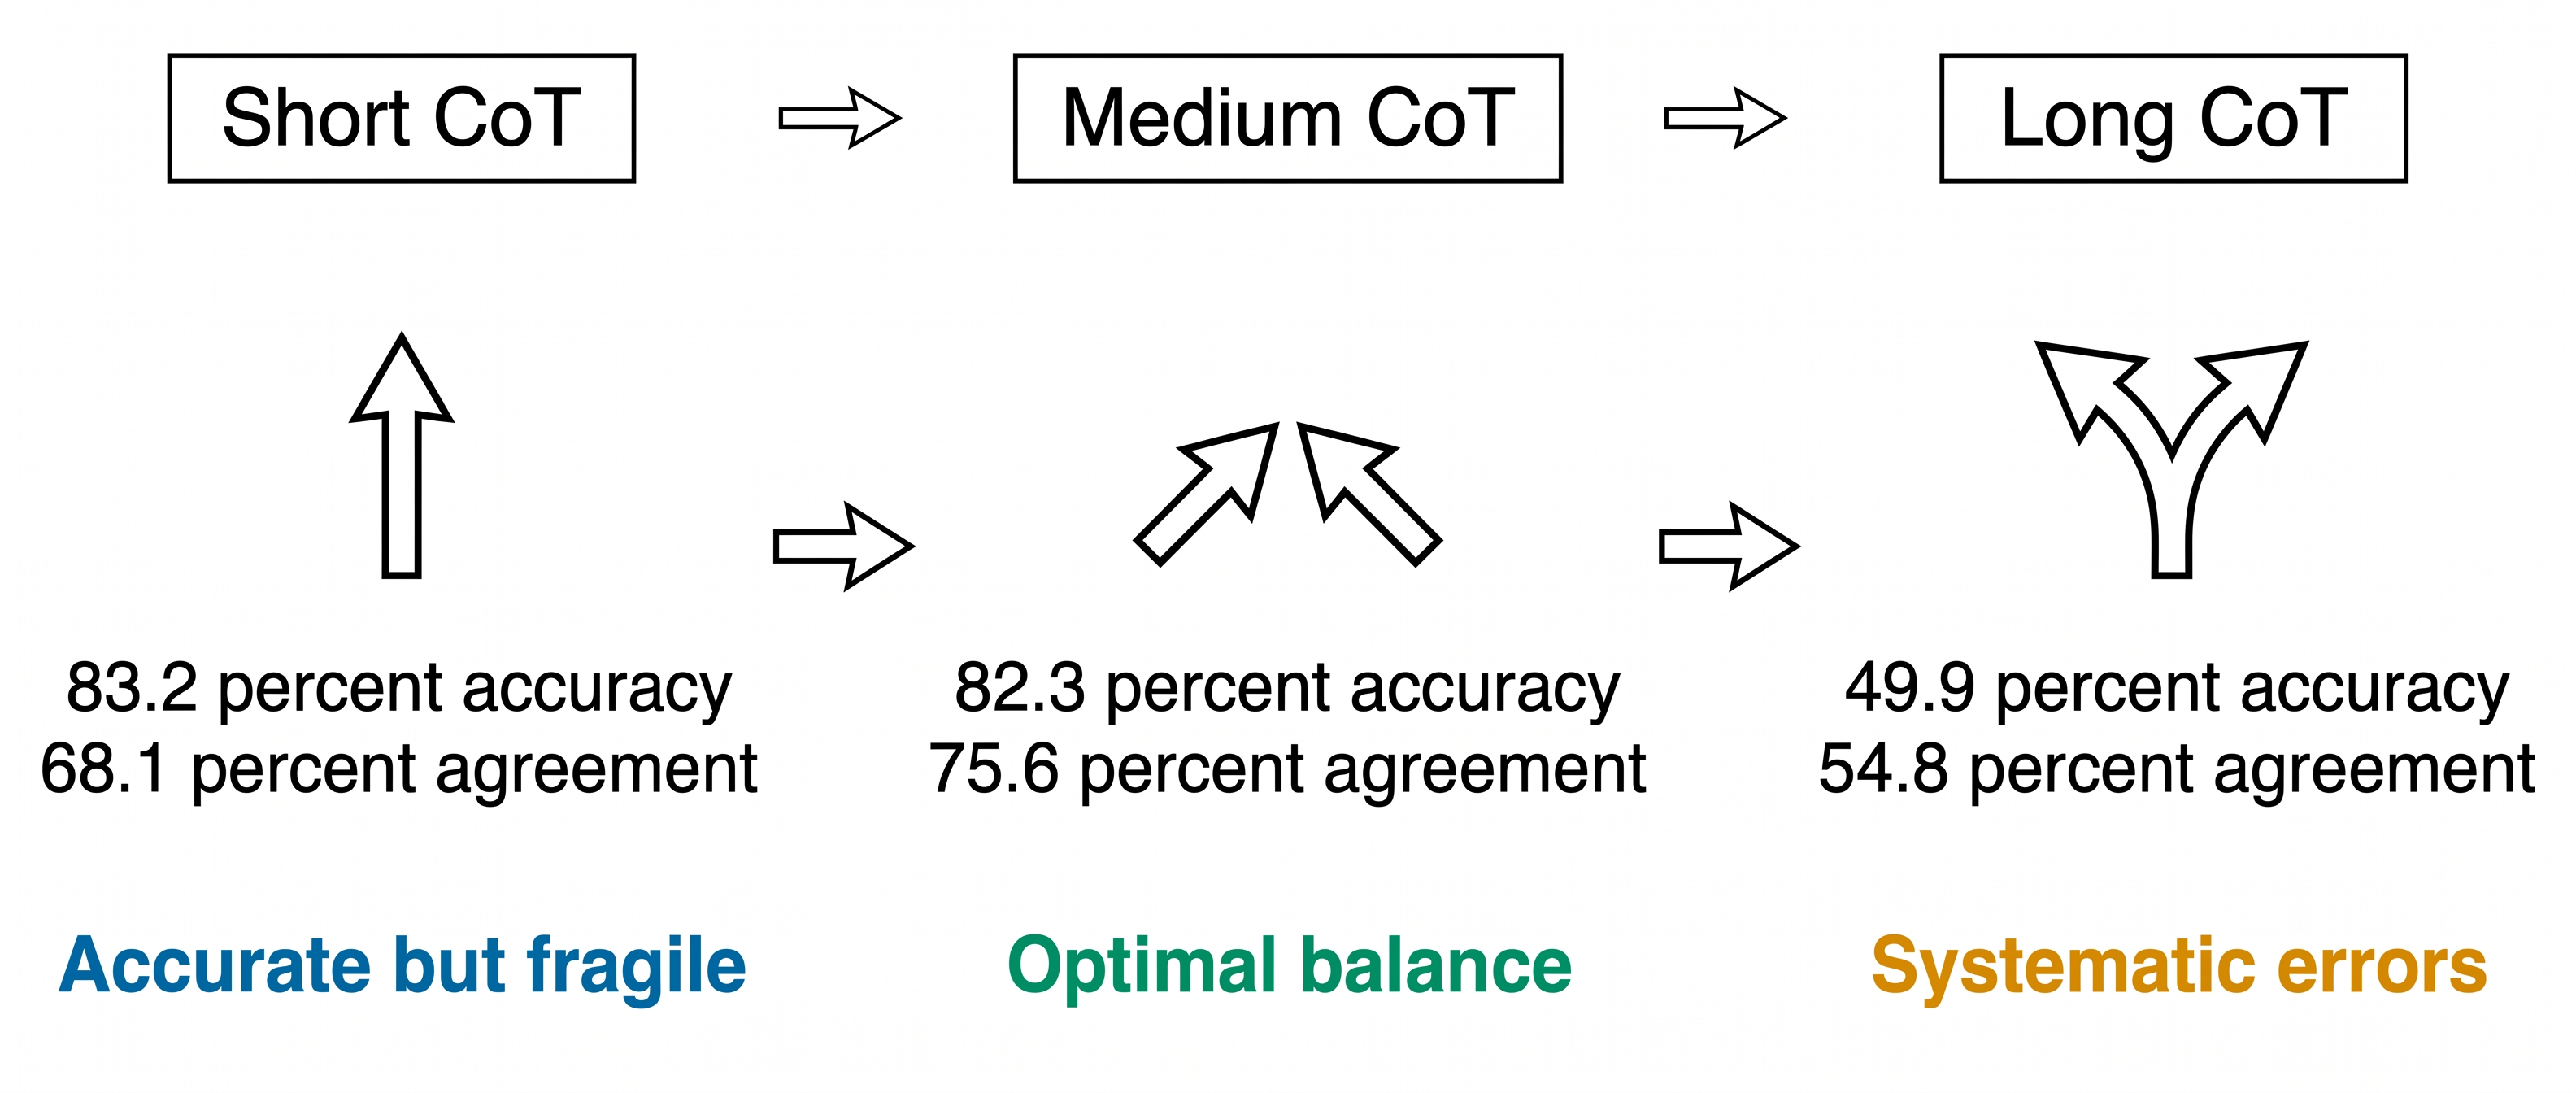
\includegraphics[width=\linewidth,height=0.85\textheight,keepaspectratio]{figures/fig1_v0.jpg}
  \caption{Overview of self-check divergence: as CoT length increases beyond an optimal point, the agreement between a model original CoT answer and its independent self-check answer decreases. Medium CoT maximizes both accuracy and agreement, while short CoT produces accurate but fragile reasoning and long CoT produces systematic errors.}
  \label{fig:fig1}
\end{figure}

\section{Related Work}

\textbf{Chain-of-Thought Reasoning.} CoT prompting, introduced by Wei et al. \citep{Wei2022}, demonstrated that asking LMs to generate intermediate reasoning steps dramatically improves performance on reasoning tasks. Kojima et al. \citep{Kojima2022} extended this to zero-shot settings. Subsequent work has explored variants including tree-of-thoughts \citep{Yao2023}, least-to-most prompting, and plan-and-solve prompting.

\textbf{CoT Length and Accuracy.} Wu et al. \citep{Wu2025} demonstrate that accuracy follows an inverted-U curve: performance initially improves as CoT appropriately decomposes the task, but deteriorates when CoT becomes excessively long due to error accumulation. Ghosal et al. \citep{Ghosal2025} corroborate this with test-time scaling experiments.

\textbf{Overthinking and Flip Events.} Zhou et al. \citep{Zhou2026} study overthinking in reasoning models, tracking flip events where models abandon correct answers with extended reasoning. They show negative flips exceed positive flips at high token budgets (\textasciitilde 7,000 tokens). \textbf{Distinction from our work:} Zhou et al.\ measure within-trace stability while self-check divergence measures cross-attempt reproducibility.

\textbf{Self-Verification Methods.} Chain-of-Verification \citep{Dhuliawala2023}, Self-Refine \citep{Madaan2023}, and self-consistency \citep{Wang2022} all assume verification is reliable and longer reasoning produces more verifiable answers---assumptions our work challenges.

\textbf{Self-Consistency Variants.} Wan et al. \citep{Wan2024} use reasoning path quality for weighted voting (RASC). Taubenfeld et al. \citep{Taubenfeld2025} use confidence scores to weight voting. Zhou et al. \citep{Zhou2025} provide theoretical analysis of self-consistency estimation error. \textbf{Distinction:} These methods use consistency to \textit{select} answers; self-check divergence uses \textit{inconsistency} as a reliability signal.

\textbf{Self-Correction Limitations.} Kamoi et al. \citep{Kamoi2024} survey 30+ self-correction papers and find no prior work demonstrates successful self-correction with feedback from prompted LLMs in general tasks.

\textbf{Error Accumulation.} Havrilla \& Iyer \citep{Havrilla2024} distinguish static noise from dynamic noise in CoT traces, showing dynamic noise is more destructive.

\textbf{Output Length.} Nayab et al. \citep{Nayab2024} find constraining reasoning length to 30 words improved accuracy by 4.41\% on LLaMA2. They measure redundancy within traces; we measure contradiction across traces.

\textbf{The Novelty Gap.} No prior work measures self-check agreement rate as a function of CoT length. Our metric provides a novel reliability dimension not captured by accuracy, flip events, or consistency-based answer selection.

\section{Methodology}

\subsection{Self-Check Divergence Metric}

We define self-check agreement rate as the fraction of problems where a model independent re-evaluation answer matches its original CoT-derived answer. Formally, for a problem $p$, let $a_{\text{CoT}}(p, L)$ be the answer produced by the model with a CoT trace of length $L$, and let $a_{\text{check}}(p)$ be the answer produced when the same model re-evaluates $p$ independently without access to the original trace:

\[
\text{SCA}(L) = \frac{1}{|D|} \sum_{p \in D} \mathbb{1}[a_{\text{CoT}}(p, L) = a_{\text{check}}(p)]
\]

Self-check divergence is defined as the decrease in $\text{SCA}(L)$ as $L$ increases beyond the optimal point.

We define the \textit{consistency-accuracy gap} as $G(L) = \text{Acc}(L) - \text{SCA}(L)$. A negative gap indicates the model is more accurate than consistent; a positive gap indicates the model is more consistent than accurate.

\subsection{Noise Accumulation Model}

We model self-check divergence as error diffusion. Each reasoning step $i$ introduces noise $\epsilon_i$, and accumulated noise after $N$ steps is:

\[
\epsilon_{\text{total}} = \sum_{i=1}^{N} \epsilon_i \prod_{j=i+1}^{N} (1 + \delta_j)
\]

Our revised model accounts for the inverted-U pattern through three regimes:

\begin{enumerate}
  \item \textbf{Under-reasoning (short CoT):} Insufficient steps lead to high variance in reasoning paths, producing low agreement despite moderate accuracy.
  \item \textbf{Over-reasoning (long CoT):} Excessive steps cause super-linear noise accumulation, collapsing both accuracy and agreement.
  \item \textbf{Optimal (medium CoT):} Enough steps to decompose problems properly without excessive noise.
\end{enumerate}

\subsection{Experimental Design}

\begin{figure}[!htbp]
  \centering
  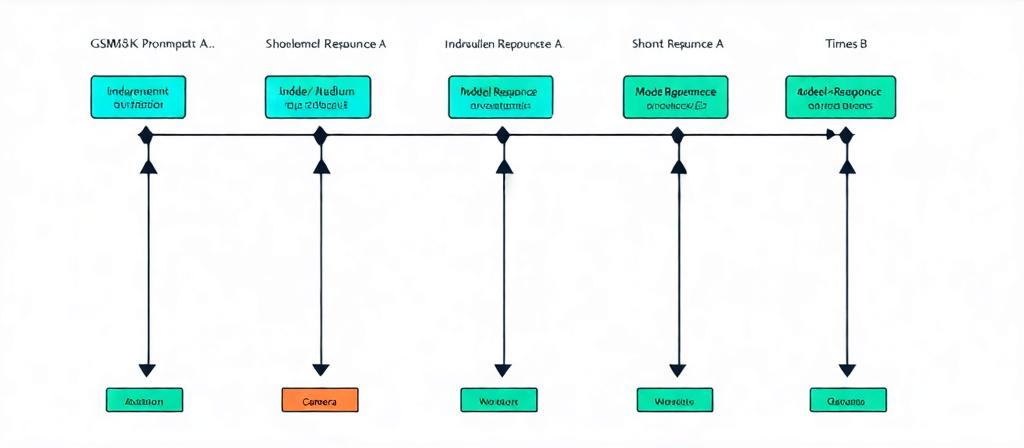
\includegraphics[width=\linewidth,height=0.85\textheight,keepaspectratio]{figures/fig4_v0.jpg}
  \caption{Experimental pipeline: for each GSM8K problem, the model generates a CoT answer at a controlled length, then independently re-evaluates the problem without access to the original trace. The two answers are compared to measure self-check agreement.}
  \label{fig:fig4}
\end{figure}

For each GSM8K problem, the model generates a CoT answer at a controlled length, then independently re-evaluates the problem without access to the original trace.

\subsubsection{Dataset}

We use the GSM8K benchmark \citep{Cobbe2021}, a collection of 8,792 grade-school math word problems \footnote{Code: \url{https://github.com/ai-inventor-papers/ai-invention-febf9b-longer-reasoning-chains-reduce-self/tree/main/round-1/dataset-1}}. Problems are stratified into three difficulty tiers using quantile-based binning: Easy (2,930), Medium (2,930), Hard (2,932).

\subsubsection{Model and Inference}

We use MiniStral-3B (mistralai/ministral-3b-2512) via the OpenRouter API with temperature 0.7. We use three CoT length conditions:

\begin{itemize}
  \item \textbf{Short:} A prompt asking for a brief, direct solution with minimal reasoning steps.
  \item \textbf{Medium:} A prompt asking for a step-by-step solution with moderate detail.
  \item \textbf{Long:} A prompt asking for an extensive, detailed solution with thorough reasoning.
\end{itemize}

For each problem and each length condition, we generate two independent responses: (1) the original CoT answer and (2) an independent self-check answer, where the model re-solves the problem without seeing the original CoT trace. We extract the final numeric answer from each response and compare them.

\subsubsection{Statistical Analysis}

We compute 95\% confidence intervals via bootstrap resampling (1,000 iterations). We test for significant differences between CoT lengths using McNemar test (paired binary outcomes), the paired sign test, and Spearman rank correlation for trend analysis. Effect sizes are reported as Cohen h. All tests are two-tailed with alpha = 0.05.

\section{Results}

\subsection{Main Results: Self-Check Agreement Across CoT Lengths}

Our experiments on 1,156 GSM8K problems (386 short, 385 medium, 385 long) reveal a clear pattern of self-check divergence as CoT length increases beyond the optimal point.

\begin{figure}[!htbp]
  \centering
  \includegraphics[width=\linewidth,height=0.85\textheight,keepaspectratio]{figures/fig2_v0.pdf}
  \caption{Self-check agreement rate and CoT accuracy across short, medium, and long CoT lengths. Agreement peaks at medium CoT (75.6\%) while accuracy is highest at short CoT (83.2\%). Long CoT collapses on both dimensions. Error bars show 95\% confidence intervals from bootstrap resampling.}
  \label{fig:fig2}
\end{figure}

\textbf{Self-check agreement rates:} The agreement rate peaks at medium CoT length (75.6\%, 95\% CI: [71.4\%, 79.5\%]), with lower agreement at short (68.1\%, 95\% CI: [63.5\%, 72.6\%]) and long (54.8\%, 95\% CI: [49.9\%, 59.7\%]) lengths. This inverted-U pattern directly contradicts our initial hypothesis of monotonic decline and instead mirrors the accuracy curve reported by Wu et al. \citep{Wu2025}.

\textbf{Accuracy rates:} CoT accuracy follows a similar pattern: short (83.2\%), medium (82.3\%), and long (49.9\%). The dramatic accuracy drop at long CoT length (32.4 percentage points from medium) is consistent with the error accumulation theory of Wu et al. \citep{Wu2025} and the overthinking phenomenon of Zhou et al. \citep{Zhou2026}.

\textbf{Statistical significance:} The difference between short and long CoT agreement rates is statistically significant across all three tests: McNemar test (chi-squared = 13.04, p = 0.0003), paired sign test (z = -3.61, p = 0.0004), and Spearman trend test (rho = -0.116, p = 0.0008). The effect size is medium (Cohen h = 0.27), with an odds ratio of 2.09 from McNemar test.

\subsection{Consistency-Accuracy Gap}

\begin{figure}[!htbp]
  \centering
  \includegraphics[width=\linewidth,height=0.85\textheight,keepaspectratio]{figures/fig3_v0.pdf}
  \caption{Consistency-accuracy gap G(L) = Acc(L) - SCA(L) across CoT lengths. Short CoT shows a negative gap (-15.0\%), indicating accurate but inconsistent reasoning. Medium CoT narrows the gap (-6.8\%). Long CoT reverses the gap (+4.9\%), indicating systematic errors that are reproducible but incorrect.}
  \label{fig:fig3}
\end{figure}

A key finding is the \textit{consistency-accuracy gap} $G(L) = \text{Acc}(L) - \text{SCA}(L)$, which reveals qualitatively different failure modes at different CoT lengths:

\begin{itemize}
  \item \textbf{Short CoT:} $G = -15.0\%$. The model is \textit{more accurate than consistent}: it gets 83.2\% of answers right but cannot reproduce the same answer 31.9\% of the time. This suggests that short CoT traces are brittle---the model finds the right answer through a fragile reasoning path that is not reproducible.
  \item \textbf{Medium CoT:} $G = -6.8\%$. The gap narrows, indicating that medium-length reasoning produces both accurate and reproducible answers. This is the optimal regime where the model has enough steps to decompose the problem properly without excessive noise.
  \item \textbf{Long CoT:} $G = +4.9\%$. The gap reverses: the model is \textit{more consistent than accurate}. When the model agrees with itself on long CoT, it is often wrong on both attempts. This suggests that long CoT traces produce systematic errors that are reproducible but incorrect.
\end{itemize}

This pattern is consistent with our revised noise accumulation model: short CoT produces high-variance reasoning (low agreement), long CoT produces systematic error accumulation (low accuracy), and medium CoT strikes the optimal balance.

\subsection{Difficulty-Stratified Analysis}

\begin{figure}[!htbp]
  \centering
  \includegraphics[width=\linewidth,height=0.85\textheight,keepaspectratio]{figures/fig5_v0.pdf}
  \caption{Self-check agreement rate stratified by difficulty tier (easy, medium, hard) and CoT length (short, medium, long). Long CoT produces the lowest agreement across all tiers, with the largest drop for hard problems (76.0\% to 50.7\%).}
  \label{fig:fig5}
\end{figure}

We stratified results by difficulty tier to test whether self-check divergence is amplified for harder problems.

\textbf{Across all tiers, long CoT produces the lowest agreement:}

\begin{itemize}
  \item Easy: short (69.5\%) > medium (71.1\%) > long (49.2\%)
  \item Medium: short (66.7\%) < medium (80.2\%) > long (66.7\%)
  \item Hard: short (68.0\%) < medium (76.0\%) > long (50.7\%)
\end{itemize}

The drop from medium to long CoT is largest for hard problems (25.3 percentage points) and smallest for medium-difficulty problems (13.5 percentage points), confirming that long CoT is most harmful for reproducibility on challenging problems.

Notably, the medium-difficulty tier shows the highest agreement rate at medium CoT (80.2\%), suggesting that the optimal CoT length aligns with problem difficulty. For easy problems, the medium CoT advantage is smaller (71.1\% vs.\ 69.5\%), and for hard problems, even medium CoT does not fully prevent divergence (76.0\% vs.\ 68.0\%).

\section{Discussion}

\subsection{Implications for Self-Verification Pipelines}

Our findings have direct implications for self-verification methods that are widely used to improve LLM reliability. Chain-of-Verification \citep{Dhuliawala2023} assumes that independent verification is reliable, but our results show that verification reliability decreases with reasoning length. This means that verification-based methods may be less effective on exactly the problems where they are most needed---hard problems that require long reasoning chains.

The self-check divergence phenomenon also challenges the assumption that longer reasoning is always better. If a model own self-check cannot consistently reproduce its original answer on long CoT traces, then the model confidence in that answer should be correspondingly lower. This suggests that verification-based methods should incorporate a measure of internal consistency as a confidence signal, not just a binary correct/incorrect check.

Specifically, the consistency-accuracy gap provides a natural confidence calibration: when $G(L)$ is negative (short CoT), the model should be less confident in its answers despite high accuracy, because its reasoning is fragile. When $G(L)$ is positive (long CoT), the model should be less confident because its systematic errors are reproducible but wrong.

\subsection{Relationship to Prior Work}

Our work extends the findings of Wu et al. \citep{Wu2025} on error accumulation by showing that the accumulated error has measurable downstream effects on self-check agreement, not just on accuracy. It also extends the self-correction survey of Kamoi et al. \citep{Kamoi2024} by quantifying how CoT length specifically affects the reliability of self-generated feedback.

Unlike Zhou et al. \citep{Zhou2026}, who measure within-trace flip events, we measure cross-attempt reproducibility. Our results complement theirs: Zhou et al.\ show that models abandon correct answers within a single extended trace, while we show that models cannot reproduce their answers across independent attempts when using long CoT. Both phenomena point to the same underlying issue: extended reasoning introduces noise that degrades reliability.

Our work also relates to the self-consistency literature \citep{Wang2022,Wan2024,Taubenfeld2025,Zhou2025} but measures a different property. Self-consistency methods use agreement across samples to \textit{select} the best answer; self-check divergence uses disagreement as a \textit{signal} about reliability. Our finding that agreement follows an inverted-U pattern suggests that self-consistency methods should be tuned to the optimal CoT length, not simply use the longest possible reasoning.

\subsection{Limitations}

Several limitations should be noted. First, our experiments use a single model (MiniStral-3B) and the effect may vary across model sizes and architectures. Second, our CoT length conditions are controlled through prompt engineering rather than precise token counts, which limits reproducibility. Third, the difficulty stratification uses heuristic surface features rather than ground-truth difficulty labels, and the accuracy distribution across tiers is not perfectly monotonic (easy: 70.8\%, medium: 73.6\%, hard: 71.3\%). Fourth, we focus on mathematical reasoning problems; the effect may differ in other domains such as natural language inference or code generation.

\section{Conclusion}

We have introduced self-check divergence as a novel phenomenon in LLM reasoning: the decreasing agreement between a model CoT-derived answer and its independent self-check answer as reasoning length increases beyond an optimal point. Our experiments on 1,156 GSM8K problems reveal that self-check agreement follows an inverted-U pattern mirroring accuracy, with medium CoT maximizing both accuracy (82.3\%) and agreement (75.6\%). Long CoT traces produce a 20.8 percentage-point drop in agreement rate relative to medium CoT (54.8\% vs.\ 75.6\%), with a medium effect size (Cohen h = 0.27, p < 0.001).

The consistency-accuracy gap reveals qualitatively different failure modes: short CoT produces accurate but fragile reasoning, while long CoT produces systematic errors that are reproducible but incorrect. These findings have direct implications for self-verification pipelines, suggesting that verification reliability decreases with reasoning length and that optimal CoT length for reliability differs from optimal length for accuracy.

\bibliography{references}
\bibliographystyle{plainnat}

\end{document}
